\begin{figure}[h]
\centering
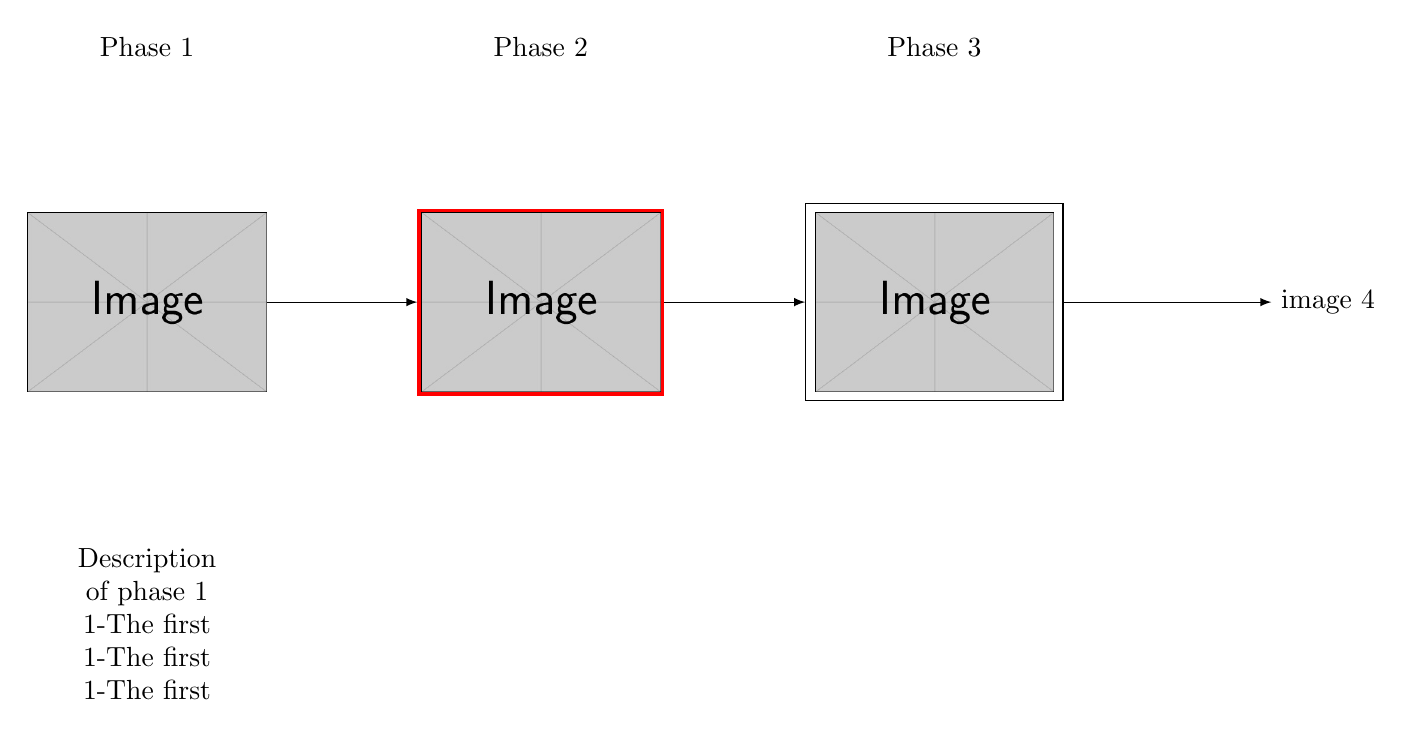
\begin{tikzpicture}[>=latex]
\node[inner sep=0pt] (n1) at (0,0) {\includegraphics[width=.25\textwidth]{example-image.jpg}};
\node[inner sep=0pt, draw, red, line width=1mm] (n2) at (5,0)  {\includegraphics[width=.25\textwidth]{example-image.jpg}};
\node[draw] (n3) at (10,0)  {\includegraphics[width=.25\textwidth]{example-image.jpg}};

\node (n4) at (15,0) {image 4};

\draw[->] (n1)--(n2);
\draw[->] (n2)--(n3);
\draw[->] (n3)--(n4);

\node[above=3cm] at (n1) {Phase 1};
\node[below=3cm, align=center] at (n1) {Description\\of phase 1\\1-The first\\1-The first\\1-The first};

\node[above=3cm] at (n2) {Phase 2};
\node[above=3cm] at (n3) {Phase 3};

\end{tikzpicture}
\label{fig1}
\caption{Project flowchart}
\end{figure}